\documentclass[a4paper,10pt]{article}
% \usepackage[utf8]{inputenc}
 
\usepackage{graphicx} 
\usepackage{langsci-gb4e}
% \usepackage{lingsty,tipa,ipashortcuts}
\newcommand{\phonet}[1]{[#1]}
\newcommand{\phonem}[1]{/#1/}
\newcommand{\graphem}[1]{<#1>}
\newcommand{\trs}[2]{\textit{#1} `#2'}
\newcommand{\tz}{ʈ}
\newcommand{\dz}{ɖ}
\newcommand{\dentt}{t̪}
\newcommand{\dentd}{d̪}

\usepackage[authoryear]{natbib}
\bibpunct[:]{(}{)}{,}{a}{}{,}
\setlength{\bibsep}{0.05cm}
%opening
\title{``Cover-up'' as a new type of contact-induced language change: Undoing the phonological history of Malay in Sri Lanka}
\author{Sebastian Nordhoff}

\begin{document}

\maketitle

\begin{abstract}
This paper establishes a hitherto undescribed sound change process which can confound diachronic reconstructions, namely ``cover-up''.  Regular sound change is contrasted with more problematic cases like loan words, doublets and reborrowings. Coverup is different from all these cases. This paper defines cover-up as the undoing of a previous sound change under influence from a contact language. Five examples of phonological cover-up from Sri Lanka Malay are given, and candidates from other linguistic domains are discussed. 
\end{abstract}


% intro SLM social history; Pali; migration %TODO
% 
% add literature %TODO
% 
% polish language %TODO
 
\section{Introduction}
Diachronic research in linguistics relies, in the absence of written documents, on comparison of related languages to establish the phonological history of the language family. Sound changes are assumed to be regular, and if a sufficiently large set of lexemes is investigated, the environments in which a certain change occurred as the proto-language developed can be established.

This relies, however, on the assumption that sound change is regular. A number of factors can distort the regular nature of sound change; one of these factors, as has been known for a long time, is language contact. Language contact can lead to new lexemes with foreign phonemes or phoneme combinations entering the language. As relevant processes, we can cite borrowings and further complications such as doublets or reborrowings, which have to be dealt with during phonological reconstruction. 

Borrowings allow us insights into past sociodemographic settings of a region. Which languages were the dominant languages in which domain? Which languages were used in in-group settings, which languages were used for wider communication? Which social group acquired another group's language? On a much more basic level, we can add ``who was where when, and who did they have what kind of contact with?'' Using the reconstructed sound changes, one can also date the transfer of lexical content from a donor language to a recipient language. The date must follow all sound changes not undergone by the lexeme in the recipient language and precede all sound changes it did undergo. This dating method is where cover-up comes into play. Cover-up undoes sound changes and thus obscures the phonological history, leading to incorrect dating of a borrowing event if the cover-up is not identified. 

This paper uses the language contact situation in Sri Lanka as a case study for cover-up.
I will first describe the linguistic situation in Sri Lanka with particular focus on Sri Lanka Malay. 
I will then give an overview of a typology of well-described lexical transfer events like borrowing and reborrowing. 
Building upon this typology, I will introduce the new concept of ``cover-up'' and show that it is different from the other processes, giving five examples from different areas of phonology such as place of articulation or syllabification. 
I will close by discussing the potential of identifying cases of cover-up in other areas of the world and in other  linguistic domains like morphology or semantics. 



 

\section{Intro SLM}
borrowing of Pali Words

migration back into the Indian sphere


\begin{itemize} 
 \item  sociodemographic history
 \item  \em who was where when, and how did the language change in the process? \em
 \item why does SLM \em gaambar \em has a long vowel while \em sambal \em has a short vowel?
\end{itemize} 
 

 



\section{Processes}
In phonological change, we can distinguish the following processes:

\begin{itemize}
    \item internal change
    \item loanwords
    \item doublets 
    \item reborrowings
    \item cover-up
\end{itemize}

The first four are well known processes. I will only briefly discuss them to provide a backdrop for the following definition of cover-up.



\subsection{Regular language change}
Regular language change is the process which is the easiest one for reconstruction: all triggers and motivations for change are internal to the language, and all items which fulfill certain conditions (phonological or syntactic environment, particular semantics, pragmatic context) change in the same way. The idea of regular change is a the source of the `unviolable sound laws' of xyz. Other languages might be spoken in the vicinity of the language which is changing, but they do not exert any influence. This is illustrated in Figure \ref{fig:regularchange}


\begin{figure} 
\centering
    
\includegraphics[height=.3\textheight]{standard.png}
\caption{Regular language change. Languages develop independently from each other}.
\label{fig:regularchange}
\end{figure}


\subsection{Loan words}
There are a number of well known processes which can muddle the clarity of the process sketched above. The first one of these is lexical borrowing. Language A takes over a lexeme from language B. The new lexeme will eventually be integrated into the phonological system of the recipient language, but might remain phonologically divergent for some time. 
%    \item \em ka\textbf{r}\em, \em b{\ae}\textbf{t}\em, \em e\textbf{kspr}es bas \em in Sinhala.

\begin{figure}
\centering
    
\includegraphics[height=.3\textheight]{borrowing.png}
\caption{The transition of a lexeme from a donor language to a target language with subsequent phonological integration}
\end{figure}

\subsection{Doublets}
A more complicated confounding factor is the presence of doublet. Doublets occur when a lexeme enters a recipient language at different points in time. While the first lexeme of a doublet can be either inherited or borrowed, the second (and further) enterings are necessarily borrowings. Examples are French \trs{nager}$<$ Latin \em navigare \em and French \trs{naviguer}{navigate}, which is also from Latin \em navigate\em, but entered the language at a later point in time. As a result, some phonological changes which occurred in \em nager\em (deletion of \em v\em, spirantization) are not found in \em naviguer\em.

This process can also occur more than twice. In Sinhala for instance, we find triplets like
\begin{itemize}
   \item  {\em yatta} ``carpenter's plane'' $<$ Sanskrit {\em yantra}
   \item {\em yatura} ``machine; key' $<$ Sanskrit {\em yantra}
   \item {\em yantraya, yantaraya\em} ``machine, talisman'' $<$ Sanskrit {\em yantra}
\end{itemize}

All of the lexemes above ultimately stem from the Sanskrit word \trs{yantra}{machine}.
The first one of these is inherited, while the second and the third are scholarly loans which occurred at later points in time. We see that language change as proceeded furthest in the first example, where the nasal and the rhotic were lost. \trs{Yatura}{key} entered the language after the gemination of muta cum liquida had already taken place. As a result, the rhotic, which was lost in \em yatta \em, remained.  In the final case, a suffix (analysed as singulative in \citet{NitzEtAl2009}) is added, which is not found in the other words. If we ignore this suffix, the Sanskrit root remains intact. 


This is illustrated in Figure \ref{fig:doublets}

\begin{figure}
\centering
    
\includegraphics[height=.3\textheight]{doublet.png}
    
\includegraphics[height=.3\textheight]{triplet.png}
\caption{Doublets entering the recipient language at three different points in time.}
\label{fig:doublets}
\end{figure}


\subsection{Reborrowing}
Another process which can obscure the regularity of linguistic changes is reborrowing. In reborrowing, a lexemes is borrowed from a donor language by the recipient language, only to be given back later to the original donor language, but with all intermittent changes. For instance the English word \em hotel \em is borrowed by Sinhala and Tamil. The meaning changed in those languages to mean \em food stall\em. The phonological shape is also |adapted, yielding \phonet{hoo{\tz}al}. This realization is borrowed back into Sri Lankan English, where it is also associated with the meaning `food stall'. Other examples of reborrowing include 

\begin{itemize}
 \item German \em Abseilen\em $\to$ English \em abseiling \em $\to$ German \em Abseiling\em `to use a rope to descend a cliff'
 \item German \trs{strafen}{punish} $\to$ WWII English {\em to maneuver a fighter plane laterally and shoot at the same time} $\to$ German \em strafen\em, \phonet{strEjfn} `to maneuver laterally in computer ego shooter games'.
 \item German \trs{\"uber}{above} $\to$ English \trs{uber}{meliorative} $\to$ German \em uber \em \phonet{ub@\;r} `meliorative'
\end{itemize}

The mechanism of reborrowing is illustrated in Figure \ref{fig:reborrowing}.

\begin{figure}
\centering
    
\includegraphics[height=.3\textheight]{reborrowing.png}
 \caption{Reborrowing}
\label{fig:reborrowing}
\end{figure}

 
\section{Cover-up}
The preceding sections have shown by which mechanisms regular sound change can be obscured. I will now turn to the main topic of this paper, cover-up. I use the following definition

\ea ``an integrated loan-word is becoming unintegrated through renewed contact with the donor language'' \z

Cover-up is thus a three stage process. The first step is the borrowing of a lexeme, the second one is the phonological integration, the third step is the undoing of the second one. p 

I will illustrate this with five examples from different domains of Sri Lanka Malay phonology. All of those have to do with a lexeme of ultimately Indic origin traveling to Indonesia, undergoing change there, traveling back to South Asia, where the change is undone. The first steps occurs during the spread of Indian culture to Indonesia via religion or trade. Indonesian languages borrowed lexemes in the course of the cultural contact, and Malay is among them. During or after the contact, some phonological changes take place. For instance, Indian languages typically have a contrast between dental and retroflex stops, and between aspirated and unaspirated stops. Furthermore, gemination is often found in Indian languages. None of this can be rendered in Malay, so that these distinctions are neutralized in the recipient language Malay. 

Typically, we are dealing with a Sanskrit or Pali lexeme, but Tamil lexemes are also found. 


\begin{figure}
\centering
    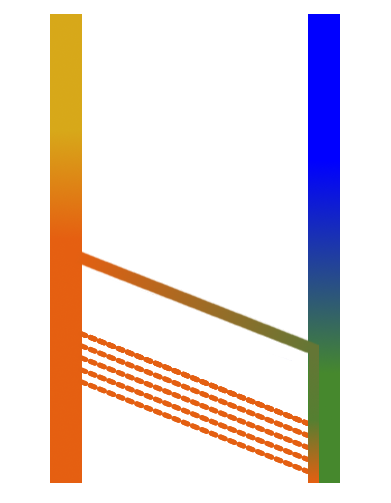
\includegraphics[height=.3\textheight]{coverup.png}
 \caption{Cover-up}
\label{fig:coverup}
\end{figure}


    

\section{Cover-up in Sri Lanka Malay}
 
\begin{itemize}
 \item  There are at least five cases of cover-up in Sri Lanka Malay
 \item Some regular sound changes are undone for lexemes which also happen to exist in Sinhala and/or Tamil
 \item Had the Malays not migrated to Sri Lanka, these sound changes would have persisted
 \item \em who was where when, and what happened in the process?\em
 \item examples: consonant length, vowel length, prenasalization, velar nasal onset, dental/retroflex stops 
\end{itemize}  

\subsection{Consonant length} 
The first case of cover-up I want to do is consonant length, i.e. a phonological contrast between short (simple) and long (geminated) consonants. Indian languages typically show this contrast, but Malay languages generally do not.\footnote{Exception
 Berau \citep{abc}.
}

Among the Indian words with geminated consonants which were borrowed into Malay, we find \trs{topi}{hat}  and \trs{kapal}{ship}. \em Topi \em is either from Hindi \em {\tz}ooppii \em or from Tamil \em toppi\em, \em kapal \em is from Tamil \em kappal\em. We see that the original lexemes showed geminate consonants, \em pp \em in this case. This gemination was, however, lost as the lexeme became integrated into the Malay language. As a result, the word \em topi \em now rhymes with \trs{sopi}{liquor}, a native word. \em Kapal \em rhymes with \em 1234\em, a native word as well. Both these lexemes entered the Malay language before migration to Sri Lanka started.

What we find today in Sri Lanka, however, is different. The words for liquor (\em soopi\em) and hat (\em {\dentt}oppi\em) do not rhyme anymore.\footnote{Sri
 Lanka Malay differs from Indonesian varieties in requiring that disyllabic lexemes have  a heavy penultimate syllable. In case the underlying form has a  CV syllable, there are two alternatives to achieve this: either the vowel is lengthened or the consonant is geminated. For more information on this, see \citet{Nordhoff2009phd}.
} 
There is no particular reason to assume that the length distinction in the consonant should be due to the difference in the onset (\em s \em vs. \em t\em). Rather, it is obvious that the presence of the adstrate Tamil with the cognate lexeme \em toppi \em led to the ``re-gemination'' of the word \em {\dentt}oppi\em. This might have been further reinforced by \em toppiya\em, the cognate in the other adstrate, Sinhala. 

The argumentation for \em kappal \em is analogous, with the exception that no cognate is found in Sinhala. 


% \includegraphics[width=.8\textwidth]{kappal.jpg} 

\subsection{Vowel length} 
A process similar to consonant happened to vowels. Indian languages often have phonemic length distinctions in vowels. Malay varieties do not. When Malay borrowed Indian words, length distinctions were neutralized. In Sri Lanka, some aspects of metrical phonology changed, which led to the reappearance of phonemic length distinctions for vowels in Sri Lanka Malay.\footnote{This
 correlates with consonant gemination: long vowels and geminate consonants cannot cooccur. See \citet{Nordhoff2009phd} for a full analysis of the metrical structure of SLM words.
}
The process of vowel lengthening is quite regular: a word of the underlying structure /CVCV(C)/ will have be rendered as [CVːCV(C)]. One exception to this rule is the word \trs{guru}{teacher}, which has a short vowel in the penultimate syllable. As words with similar environments like \trs{{\dentt}uurung}{descend} behave in a regular way, the question as to the exceptional status of \em guru \em arises. Things get again clearer when we look at the adstrates: Sinhala has \em guruvarayaa \em  with a short vowel. Cover-up again provides an explanation for the exceptional behaviour of \em guru\em: the presence of an adstrate with a cognate to the original loan led to the undoing of the regular vowel lengthening process. One could argue that the word \em guru \em actually never underwent the vowel lengthening process, and that in that case, we would not be dealing with cover-up, but rather with some kind of blocking. Data from Jakarta Indonesian, however suggest that vowel lengthening had already started back in Indonesia, but
without becoming phonemic there. Jakarta was the port of embarkation from where the immigrants to be soldiers left for Sri Lanka. Jakartan varieties have been identified as the main input for Sri Lanka Malay, next to Moluccan varieties \citep{Paauw}. In Jakarta Malay, we find the lengthening of the penultimate syllable of a phrase \citep{abc}. This suggests that the vowel lengthening processes already started in Indonesia, for both \em {\dentt}uurung \em and \em guuru\em, but that the change for the latter lexeme was undone upon contact with Sinhala. 


\subsection{NC clusters} 
The third domain of cover-up has to do with the syllabification of NC clusters. We can distinguish heterosyllabic N.C clusters from tautosyllabic .NC clusters. In Sri Lanka Malay, the tautosyllabic clusters are much more common. We find \trs{gaa.mbar}{picture} 
$<$ \em gambar\em, 
\trs{{\dentt}aa.ndZak}{dance} $<$ \em tandak \em, 
\trs{baa.njir}{flood} $<$ \em banjir \em, 
\trs{{\dentt}ii.nggi}{tall} $<$ \em abc\em. Syllabification of NC clusters in Indonesian varieties of Malay can follow one pattern or the other. Heterosyllabic clusters are found in words starting with a vowel \trs{am.bel}{take} and \trs{anjing}{dog}. For those, a phonological explanation might be available. But for the word \trs{sam.bal}{spicy dish}, no such explanation suggests itself. It is very similar to the word \trs{gaa.mbar}{picture}, but still, the syllabification is different. Again, the
adstrates provide an explanation: both Sinhala \em sam.bol \em and Tamil \em sam.bal \em show a heterosyllabic syllabification and a short vowel. `Sambal' is an emblematic dish of Indonesian culture, and it is clear that this concept has been in common everyday use for centuries. It can therefore be excluded that \em sambal \em is a recent loan from Sinhala or Tamil. Rather, it is a word which was in use among the immigrants, and which obeyed the same metrical constraints as other words like \em gaa.mbar\em. Only upon contact with Sinhala and Tamil did this change, and the standard tautosyllabic syllabification was changed to heterosyllabic.

\subsection{Syllabification of {\ng}} 
Yet another example where syllable structure plays a role is the syllabification of {\ng} in the word for `lion'. Malay borrowed the Sanskrit word {\em si{\ng}.ha} for this concept. {\em Si{\ng}.ha} has a coda {\ng} in the penultimate and an onset \em h \em in the final syllable. The h was dropped in Malay, and the velar nasal resyllabified to the onset of the final syllable, yielding the form \em si.nga\em, which is what is still found today in Indonesia. This lexeme is then similar to other words, like \trs{i.ngat}{think} or \trs{di.nging}{cold}. In Sri Lanka, words of this structure underwent the vowel lengthening processes described in Section \ref{abc}, leading to \trs{{\dz}ii.nging}{cold} and \trs{ii.nga{\dentt}}{think}. But such was not the case for \em si.nga\em. Here, syllabification of {\ng} changed yet again, and what we find in Sri Lanka Malay is \em sing.ga\em. Note that the Sri Lanka Malay word has reinstated the coda in the first syllable and the onset in the final syllable, albeit a voiced velar stop instead of the uvular fricative which was present in Sanskrit. The explanation for this comes as no surprise: both Sinhala ({\em si{\ng}.ha.yaa}) and Tamil ({\em si{\ng}.gam}) have a cognate with a coda and an onset. Again, there is no reason to assume that Sri Lanka Malay would have borrowed the Sinhala or the Tamil word. Rather, the native word was made to conform to what is found in the adstrates, and preceding phonological changes, here the syllabification of {\ng} were undone.

\subsection{dental$\to$alveolar$\to$dental} 
The final change which I want to discuss under the rubric of cover-up is the realization of the voiced coronal stop. In Indian languages, there is normally an opposition between dental and retroflex points of articulation. This difference does not exist in Malay. In loanwords, this distinction is neutralized, and all voiceless coronal stops of Indian loan words become dental and all voiced ones, alveolar. This is for instance what happened to the Tamil word \trs{kalu{\dentd}ai}{donkey}. Malay borrowed this word as \em keldai\em, with an alveolar d. In Sri Lanka, all medial voiced coronal stops were retracted and are now retroflex. An example would be \trs{laa{\dz}a}{pepper} $<$ \em abc\em. A dental voiced stop can only be found in initial position and in Arabic loanwords. And in the word for donkey, which is \em kal{\dentd}e\em. This is due to renewed exposure to the Tamil lexeme and its dental articulation. As with the other examples, it is clear that \em kalde \em is not a direct loan from Tamil. The concept was in use all the time, and the phonological shapes are too different. Rather, the word \em keldai \em with alveolar articulation was brought from Indonesia, but the alveolar articulation was changed back to dental upon contact with Tamil, the language change was undone. 


\subsection{Summary} 
\begin{itemize}
 \item ``an integrated loan-word is becoming unintegrated through renewed contact with the donor language''
 \item examples mainly from metrical phonology (quantity distinctions, syllabification)
 \item one more phonetic example (dental {\dentd})
\end{itemize} 

\subsection{Problems} 
The main problem in the area of cover-up is how such cases can be distinguished from plain new loans. One could argue that a word like \em kapal \em was dropped first, and later \em kappal \em was borrowed into a clean slate language. Similar arguments are available for the other cases mentioned. However, for the examples cited in this paper, the continuity of the lexemes \em kapal, topi, guru, singa, kalde \em is a sensible assumption because of their frequent occurrence in daily life. Living in a tropical island requires frequent use of boats and hats, and religion and myths make sure that the concepts of `teacher' and `lion' are used on a regular basis. The case for `donkey' is a bit weaker. For all these lexemes, however, the absence of synonyms suggests that they were used all along. If they had fallen into disuse, only to be borrowed again in Sri Lanka, we would expect to find traces of the former words, possibly with some semantic shift. Of the lexemes discussed in this paper, no such instances are known. For the cases discussed here, we can therefore be confident that we are indeed dealing with cover-up, and not with new loans. 



\subsection{Cover-up elsewhere}
So far, we have concentrated on phonology. The reason for this is that phonological change is much more regular than semantic or syntactic change for instance, and that we can make reasonable assumptions about which outcome would be expected for a given environment. This is much more difficult for other subdomains of linguistics. Another reason is that in order to find morphological or syntactic cover-up, one must be able to identify cases of morphological or syntactic borrowing in the first place. While morphological borrowing is easy to identify, it is not a very frequent phenomenon, meaning that a rather extraordinary process like cover-up is not easy to find among the few documented cases of morphological borrowing. Syntactic cover-up suffers the problem of the limited power of syntactic reconstruction. It is much more difficult for syntax than for phonology to trace the evolution of a particular item, or to exactly identify the point in time when calquing took place.
Of all other subdomains of linguistics, lexical semantics seems to be most promising. There are number of borrowings (or `pseudo-borrowings') of English lexemes into German, which underwent semantic change when being borrowed. These include \em beamer \em (`projector'), \em body bag \em (`backpack'), and \em controlling \em (`managerial accounting'). It is conceivable that prolonged and intensified contact to English will eventually lead to these semantic shifts being undone and to the lexemes reverting to their original senses.
However, for these cases, it would be even more difficult to distinguish cover-up from a fresh loan than in phonology. If Germans use the word \em body bag \em in 20 years from now for a container for corpses, would we think that this is a semantic shift from \trs{body bag$_{1}$}{back back} to \trs{body bag$_{2}$}{container for corpses}, or would we rather say that \em body bag$_{1}$ \em was lost and \em body bag$_{2}$ \em is a new loan?

Finally, orthography might be a candidate for cover-up. This can be illustrated with an anecdotal example. When eliciting the word for `earth', \em buumi\em, a Sri Lanka Malay consultant insisted it should be written with the Sinhala letter \graphem{bh}. This was completely surprising, as Sri Lanka Malay does not have distinctive aspiration, and neither do Sinhala or Tamil. However, Sinhala orthography maintains the distinction, and there are a couple of Sanskritisms where the use of the graphemes for the aspirated stops is required. \graphem{bhumiya} is one of them. The consultant made the transfer of Sinhala orthography requiring a \graphem{bh} for this concept to Sri Lanka Malay phonology, thereby undoing the neutralization of aspiration as a distinctive feature in Malay. This was obviously only possible because of his knowledge of Sinhala orthography, which led to a renewed contact with an offshoot of the original donor language, Sanskrit.

\subsection{Conclusion} 
In this article, I have sketched a new type of sound change, cover-up, which has to be dinstinguished from regular change and borrowing. I have given five examples from different domains of phonology. Cover-up is only possible when two contact situations are separated by a long period without relevant contact. Furthermore, cover-up can most likely only be identified in phonology. These conditions mean that it is not a very frequent process, but still one which is theoretically very interesting.
The main issues for future research are the identification of other language contact situation where cover-up has taken place, a clearer distinction between cover-up and new loan, and the investigation of whether cover-up can be found in other domains of linguistics.  



\bibliographystyle{natuva}
\bibliography{nordhoff}


\end{document}
